\chapter{Premiers pas}\label{chap:premiersPas}


\TCBimportant{Même si vous n’avez pas l’intention d’utiliser le site par la suite, il est indispensable de suivre la procédure décrite dans la première section intitulée \og{}Activation du compte\fg{} sinon votre compte ne sera pas validé et vous ne recevrez aucun message (offres, demandes, etc.) de la part de votre \sel.}

\section{Activation du compte}

Vous avez reçu un message semblable à celui de la figure \ref{fig:messageInformation} (\vpageref{fig:messageInformation}) adressé à Charlotte \textsc{Arnaud}\footnote{Charlotte est une adhérente factice créée pour les besoins de ce tutoriel.}.
Il signale que votre compte a été créé par un \index{administrateur local}administrateur local; il vous appartient maintenant de l’activer.

Seules les deux lignes surlignées en jaune ou en vert nous intéressent.
\begin{figure}
    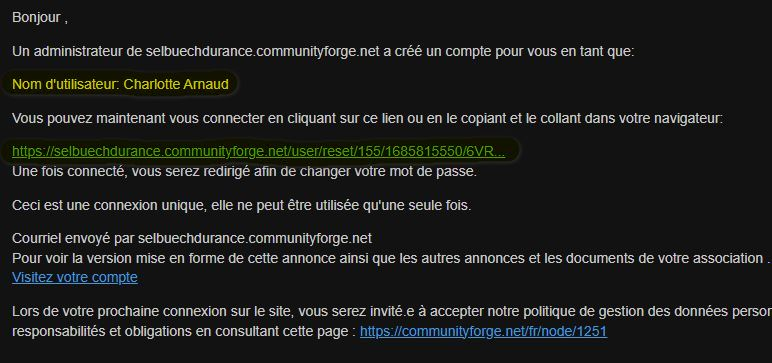
\includegraphics[width=\linewidth]{006-message_d_information}
    \caption{Message d'information (création du compte)}
    \label{fig:messageInformation}
\end{figure}
\begin{figure}
    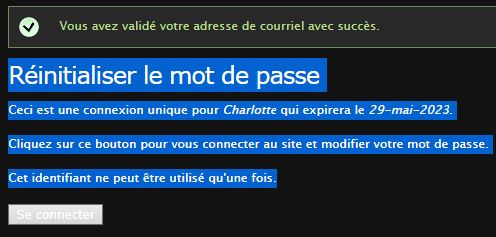
\includegraphics[width=\linewidth]{010-reinitialiser_mdp}
    \caption{Réinitialiser le mot de passe}
    \label{fig:reinitialiserMdp}
\end{figure}
\begin{figure}
    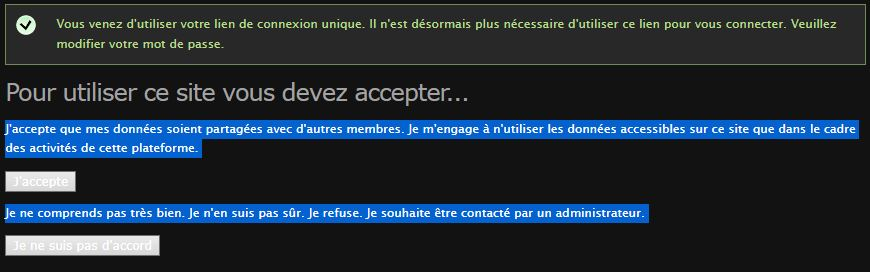
\includegraphics[width=\linewidth]{020-accepter_RGPD}
    \caption{Accepter le RGPD}
    \label{fig:accepterRgpd}
\end{figure}
\begin{enumerate}
    \newcounter{noteProfilPasAJour}
    \item Notez votre nom d’utilisateur (ligne surlignée en jaune), normalement votre prénom et votre nom --- si votre nom ne figure pas, il faudra effectuer une mise à jour de votre \index{fiche de profil}profil pour l'ajouter (voir la section \og{}Onglet Mes infos\fg, p. \pageref{page:completerInfosPerso})%
    %%%
    \footnote{\setcounter{noteProfilPasAJour}{\value{footnote}}\label{page:profilPasAJour}\index{Profil!mise à jour}Certaines captures d'écran ont été faites avant que le profil de Charlotte \textsc{Arnaud} ait été mis à jour, si bien que seul le prénom apparaît (voir figure  \vref{fig:reinitialiserMdp}, et de nombreuses autres figures, notamment Fig. \ref{fig:menuUtilisateur}, p. \pageref{fig:menuUtilisateur}).}.
    %%% 
    \item Cliquez sur le lien surligné en vert ou recopiez-le dans la barre d’adresse de votre navigateur ---  ce lien n’est utilisable qu'une fois, nous verrons plus loin  comment se connecter par la suite.
    \item Vous arrivez sur la page de la figure \ref{fig:reinitialiserMdp} (\vpageref{fig:reinitialiserMdp}).
    \item Cliquez sur \autresliens{Se connecter} pour ouvrir la page de la figure \ref{fig:accepterRgpd}.
    \item Cliquez sur \autresliens{J’accepte}\index{RGPD}\label{page:accepteRgpd}%
    %%%
    \footnote{Vous avez le droit de ne pas accepter, pour cela, cliquez sur \autresliens{Je ne suis pas d'accord} au lieu de \autresliens{J'accepte}, vous resterez membre du \sel mais vous ne pourrez pas utiliser le site et surtout vous ne recevrez pas les courriels (offres, demandes, actualités, etc.).}
    %%% 
    ce qui ouvre une nouvelle page (Fig. \vref{fig:choisirMdp})
    \item Choisissez un mot de passe puis confirmez-le.\index{mot de passe!définir}
    \item Enfin, \textbf{n’oubliez pas une dernière étape indispensable}: descendez tout en bas de la page et cliquez sur le bouton \autresliens{Sauvegarder}, non visible à la figure \ref{fig:choisirMdp} (mais visible Fig. \ref{fig:pageParametres}, p. \pageref{fig:pageParametres}).
\end{enumerate}

\medskip

\begin{center}
    \textbf{Votre compte est maintenant activé}
\end{center}

\rem{\index{mot de passe!choisir un bon}\CF{} ne n'impose aucune contrainte pour le choix du mot de passe, il  est cependant conseillé de respecter quelques règles; vous trouverez à cette adresse:}
\index{Cnil@\textsc{Cnil}}
\begin{center}
    \liensdirects{\small https://www.cnil.fr/fr/les-conseils-de-la-cnil-pour-un-bon-mot-de-passe }
\end{center}
\begin{figure}
    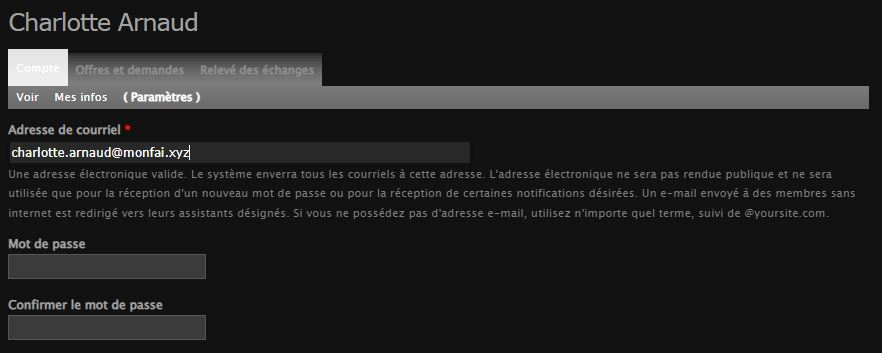
\includegraphics[width=\linewidth]{031-page_utilisateur}
    \caption{Choisir un mot de passe}
    \label{fig:choisirMdp}
\end{figure}
\medskip
les conseils de la \textsc{Cnil} pour le choix d’un bon mot de passe%
%%%
\footnote{Il va sans dire que ces conseils valent pour tous vos mots de passe, pas seulement sur \CF.}.
%%%

\section{Première connexion}

Allez sur le site du \CdS à l’adresse%
%%%
\footnote{À l'origine, le site était commun à trois \sel, \CdS, \sel des 3 Rivières de Sisteron et Galet du Buech de Laragne, d'où le nom du site \texttt{selbuechdurance} qui les réunissait tous les trois.}:
%%%
\begin{center}
    \liensdirects{https://selbuechdurance.communityforge.net/}
\end{center}

\medskip

\begin{figure}
    \centering
    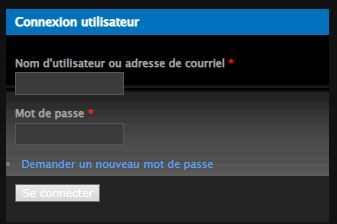
\includegraphics[width=.7\linewidth]{040-ecran_de_connexion}
    \caption{Écran de connexion}
    \label{fig:ecranConnexion}
\end{figure}
\index{se connecter}
En haut à droite, se trouve un formulaire de connexion très classique (Fig. \ref{fig:ecranConnexion}) où entrer votre identifiant et le mot de passe que vous avez défini lors de l’activation du compte, avant de cliquer sur \autresliens{Se connecter}.

La seule petite subtilité de ce formulaire concerne l’identifiant qui peut être soit (de préférence) votre adresse courriel --- \texttt{charlotte.arnaud@monfai.xyz} dans notre exemple ---, soit votre nom tel qu’il est enregistré sur le site ---  ici Charlotte \textsc{Arnaud}.

\index{se connecter!deux identifiants possibles}
\rem{Parfois, en cas de difficultés avec un des identifiants, l’autre méthode peut résoudre le problème.}

\subsec{Mot de passe oublié}\label{sec:mdpOublie}
\index{mot de passe!réinitialiser}
Si vous avez oublié votre mot de passe, il est possible de demander sa réinitialisation en cliquant sur \autresliens{Demander un nouveau mot de passe} (Fig. \ref{fig:ecranConnexion}). Suivre ensuite une procédure assez semblable à celle décrite ci-dessus sauf que vous n’aurez, notamment, plus à accepter le RGPD%
%%%
\footnote{Brièvement, vous recevrez un nouveau lien de connexion à usage unique (semblable à celui de la figure \ref{fig:messageInformation}), il faudra ensuite définir un nouveau mot de passe (Fig. \ref{fig:choisirMdp}) et enfin cliquer sur \autresliens{Sauvegarder} en bas de la page.}.
%%%

\rem{En  cas de difficultés, contactez-moi, je vous attribuerai un mot de passe provisoire que vous pourrez ensuite changer (voir section \og{}Changer le mot de passe\fg, p. \pageref{sec:changerMotDePasse}).}

\section{Où trouver les premières informations ?}\label{page:premieresInfos}

\index{page d'accueil}La page d’accueil du site est la page \noncliquables{Actualités} (voir chapitre \ref{chap:descriptionPage} <<~Brève description d’une page~>>). Rendez vous à la dernière page --- il faudra peut-être cliquer sur \autresliens{Suivant}  en bas de la page jusqu’à atteindre la dernière ---, pour y trouver le guide rédigé par Arno%
%%%
\footnote{Arno a été le premier administrateur local du site du \CdS; il n'est plus membre du \sel{} aujourd'hui.} 
%%%
lors de la création du site. Il n'est pas exhaustif mais il est suffisant pour l’essentiel des usages%
%%%
\footnote{Le début de ce guide apparaît à la figure \ref{fig:vueGeneralePage}, p. \pageref{fig:vueGeneralePage}}.
%%%

\index{FAQ}
Une Foire aux Questions, lien \liensmenu{FAQ} du petit menu situé en haut à droite de la \index{page d'accueil}page d’accueil (\index{menu secondaire}menu secondaire, voir \vref{sec:menuSecondaire}), vous apportera aussi des informations utiles. \rem{Notez toutefois que cette \textsc{Faq} rédigée par l’équipe de \CF{} décrit l'ensemble des fonctionnalités du site qui ne sont pas toutes utilisées au \CdS{} --- en particulier, nous consignons les échanges sur le carnet papier et non sur le site.}

Enfin, toujours dans le même menu secondaire, le lien \liensmenu{Docs}\index{Docs} permet l’accès à plusieurs documents classés par rubriques. Une  des rubriques est intitulée \noncliquables{Tutoriels}. Pour l’instant, elle est vide, je vais essayer de l’alimenter dans le futur --- la rédaction de tutoriels est assez longue, je ferai en fonction du temps que j'aurai.
